\chapter{Introduction}
\label{cha:intro}

%\section{Spatial cognition and probability}
%\label{sec:intro:brainspaceprob}

Brains have evolved to move bodies through space in order to increase the chances of survival and reproduction, through numerous complex behaviours such as fleeing from threats or searching for nutrients or potential mates. The ability to remember spatial information, e.g. previously encountered food sources or shelters, has provided sufficient evolutionary advantage that all known organisms with brains (and even some without, such as the slime mold\footnote{Slime molds are able to avoid previously explored areas using externalized spatial memories, and to solve mazes using nutrient gradients} - \citet{reid2012slime}) have at least a rudimentary ability to utilize representations of space for more efficient navigation. Higher mammals have evolved a network of brain areas implementing spatial memory, a system for storing and recalling spatial information about the environment and about their location in it.

Representing spatial information accurately in the real world is hard, for several reasons. Sensors and actuators are limited, erroneous and noisy (in the sense of noise interfering with the signal). There are additional sources of uncertainty or unknown information, such as external events, actions of other organisms, unperceived or currently unperceivable objects or events. Furthermore, physical environments can be highly complex, and yet cognitive resources (amount of memory, processing power, time and energy available) are necessarily limited by biological and physical constraints. 

In artificial intelligence (AI) and robotics research, probabilistic models have provided key tools for dealing with such challenges, facilitating the quantitative characterization of beliefs and uncertainty in the form of probability distributions, and the machinery of Bayesian inference for updating them with new data. They have also inspired the `Bayesian brain' \citep{knill2004bayesian} and `Bayesian cognition' \citep{chater2010bayesian} paradigms in the cognitive sciences. These paradigms have been successful in explaining human behaviour in tasks as diverse as the integration of sensory cues \citep{ernst2006bayesian} including spatial information \citep{cheng2007bayesian,nardini2008development}, sensorimotor learning \citep{kording2004bayesian}, visual perception \citep{yuille2006vision} or reasoning \citep{oaksford2007bayesian}. Their success suggests an answer to what biological cognition might be doing to cope with the above-mentioned challenges: approximate Bayesian inference.

%\begin{figure}[h]
%	\centering
%	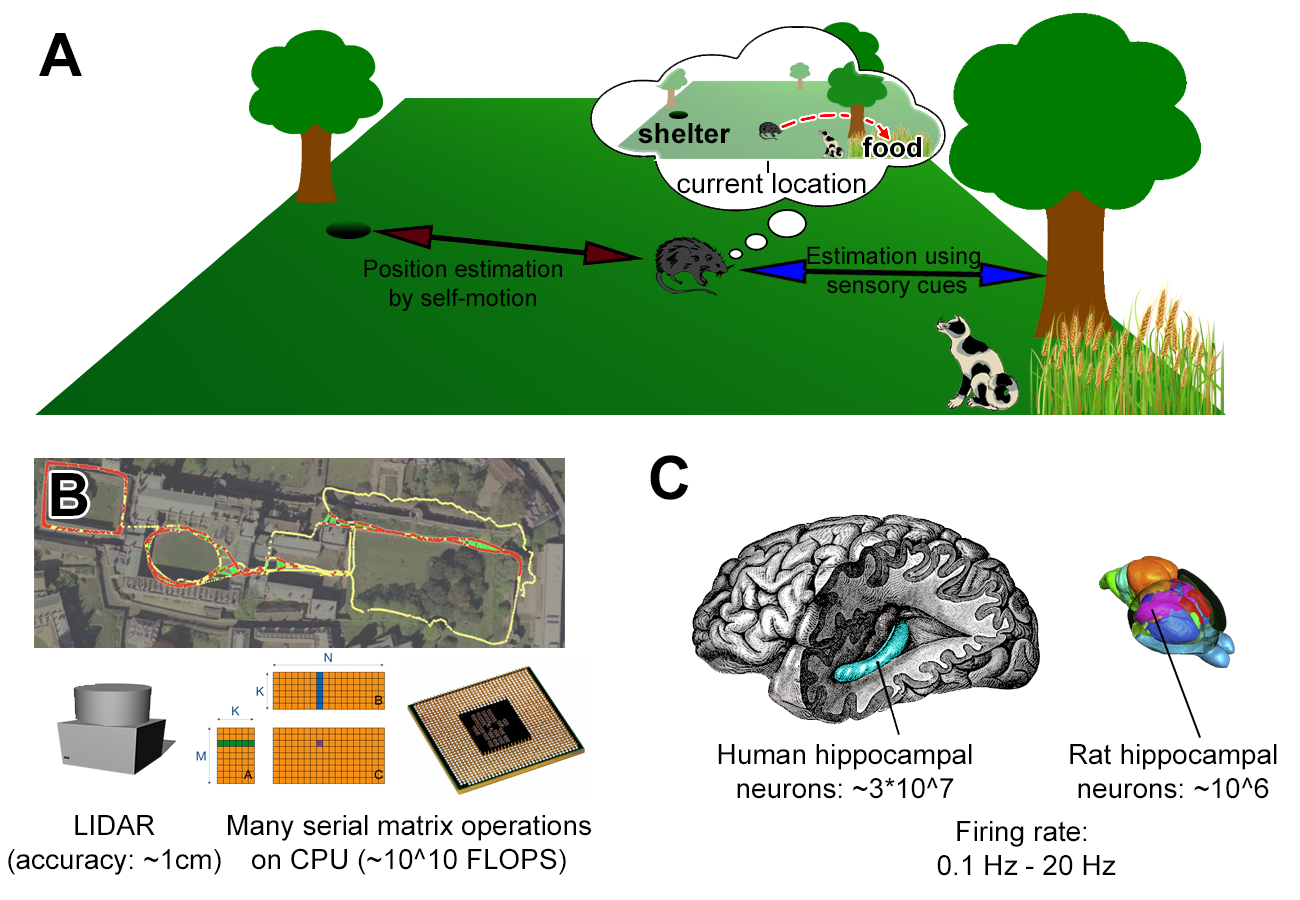
\includegraphics[width=\textwidth]{img/motivation}
%	\caption{\textbf{Motivation for proposing new computational cognitive models of spatial memory}. A: Learning representations of the space around animals confers significant advantages, such as the ability to plan a detour (dashed red arrow) to reach a food source while avoiding danger in this example (not trivial if the goal and detour are out of sight). In real environments, this task is made more difficult by the unreliability, errors and noise inherent in both the estimation of position by integrating self-motion, or by estimated object distances (e.g. based on vision). Most existing cognitive models of spatial memory neglect these challenges. B: State of the art SLAM models in robotics are able to estimate locations and learn maps accurately, but rely on sensors and computations which are very different from biology - e.g. higher measurement accuracy using laser-based distance sensors (LIDAR), centralized control and coordination, and high number of serial operations per second - up to $10^{10}$ floating-point operations per second (FLOPS) needed for state of the art SLAM systems \citep{machado2013evaluation}. C: In contrast, the hippocampus - the major brain area involved in world-centered spatial representations - contains only a few million neurons firing only a few times per second \citep{rapp1996preserved,vsimic1997volume}; and relies on noisy, inaccurate sensory measurements. Although many models of spatial memory in brains exist, there is a lack of computational mechanisms which are both neurally and psychologically plausible, and can work in realistic environments and with noisy sensors. (Example SLAM data in Panel B from \citep{newman2011describing}, and 3D rat brain from \citep{calabrese2013ontology}, with permission.)}
%	\label{fig:motivation}
%\end{figure}
%
\section{Motivation}
\label{sec:intro:motivation}

Despite of this success and of the suitability of probabilistic models to deal with uncertain and noisy spatial information, there have been few attempts to use them for modelling spatial memory within cognitive modelling, the branch of cognitive science concerned with computationally simulating mental processes. There is a gap in literature between probabilistic spatial models in robotics (called Simultaneous Localization and Mapping or SLAM) \citep{thrun2008simultaneous}, which are capable of dealing with real-world noise, uncertainty, and complexity to some extent, but are cognitively implausible\footnote{In our usage of the terms, a computational model is `psychologically plausible' (or `cognitively plausible') to the extent that it is consistent with psychological findings and can accurately reproduce psychology data, i.e. behaviours. Analogously, it is `biologically plausible' (or `neurally plausible') to the extent that it is consistent with neuroscience and can reproduce neural data, e.g. single-cell recordings or brain imaging results.}, and between computational cognitive models of spatial memory, which are designed to model biological spatial cognition, but cannot deal with all of these challenges, and are thus confined to simplistic simulations (see Chapter TODO for a review). 

%There is also a dearth of models of \textit{how} neurons could be able to perform Bayesian inference to improve spatial representations, and of evidence on a neuronal level (as opposed to behavioural) that they can. 

In addition, although spatial representations in humans have been argued early to be hierarchical \citep{hirtle1985evidence, mcnamara1989subjective, wiener2003fine}, similarly to some robotic implementations having to deal with large, complex environments \citep{kuipers2000spatial, wurm2010octomap}, it is not known how (by which process) these hierarchical spatial maps might be structured. Although many computational models of spatial memory running in simplified environments exist, there is a lack of biologically and psychologically plausible `algorithms' serving as models of human cognitive computations related to spatial information processing which can function in realistic, uncertain, complex environments.

The deprioritization of the problems of uncertainty and noise in favour of tractably modelling other human cognitive mechanisms is also pronounced in cognitive architectures, which try to account for a large number of mental processes in a unified, comprehensive, systems-level model (as opposed to computational cognitive models, which usually focus on a single phenomenon). In their overview of the field, \cite{langley2009cognitive} argue that \textit{`` we should attempt to unify many findings into a single theoretical framework, then proceed to test and refine that theory''}, supporting the arguments of \cite{newell1973you} that \textit{``you can't play 20 questions with nature and win''}, highlighting the importance of systems-level research in the cognitive sciences. Although a few such cognitive architectures do model spatial mechanisms in navigation space \citep{harrison2003act,schultheis2011casimir,sun2004top}, they all run in simple, noise-free environments. According to a comparative table of cognitive architectures \citep{samsonovich2011comparative} available in updated form online\footnote{http://bicasociety.org/cogarch/architectures.htm}, there is currently no cognitive architecture implementing both Bayesian update and an empirically validated `cognitive map' at the same time\footnote{CogPrime \citep{goertzel2013cogprime} claims to implement both Bayesian update and cognitive maps, but neither of these mechanisms have been evaluated against human data, or indeed claim to be modelling human cognitive phenomena at all. Instead, CogPrime aims for artificial general intelligence, as opposed to closely adhering to human cognition.}.

The present work was motivated by these gaps in literature, and aims to take computational cognitive models of navigation-scale\footnote{Human cognition needs to keep track of the space of navigation as well as the spaces immediately around the body (e.g. reachable objects) and of the body (e.g. body-part configurations). Although uncertainty and noise play are important in the latter two spaces as well, we will confine ourselves to navigation-scale spatial mechanisms in this work.} spatial memory one step closer to modelling behaviour in realistic environments, such as high-fidelity robotic simulations or physical environments, by means of proposing probabilistic mechanisms of spatial cognition which are implementable in brains and can reproduce behaviour data. Situated within cognitive modelling and cognitive architectures, the goal of this work is to contribute to the understanding of information processing in human cognition. As such, although it is computational in nature, the extent of its success is determined by its ability to predict and explain the kinds of behaviour data it is intended to model, as well as its consistency with established findings in psychology and neuroscience. It is not aiming for performance, or accuracy of learned spatial representations (these are the domains of robotics), or for maximizing neurobiological fidelity at the cellular level or below. Although building on neuroscientific evidence, our concern is modelling spatial information processing on Marr's algorithmic level of analysis \citep{marr1976understanding, marr1977understanding}, as opposed to e.g. biological neural networks - see Table \ref{tbl:marr} -, with a single exception. 

\begin{table*}[h]
	{\renewcommand{\arraystretch}{1.2}
		\begin{tabu}{c|c|c}
			$\downarrow$ {Level of analysis} & {Description} & {In this work}\\ \tabucline[3pt]{-}
			1. Computational & \begin{tabular}[c]{@{}c@{}} What problem(s) does the \\ system solve, and why? \end{tabular} & \begin{tabular}[c]{@{}c@{}} Localization,\\ Map error correction, \\ Map structuring \end{tabular} \\\hline
			\begin{tabular}[c]{@{}c@{}} \textbf{2. Algorithmic/} \\ \textbf{Representational} \end{tabular} & \begin{tabular}[c]{@{}c@{}} How might it solve them? (Using\\ what representations and processes?) \end{tabular} & \begin{tabular}[c]{@{}c@{}} Cognitive models \\ of spatial memory \end{tabular} \\\hline
			3. Implementation & How is it implemented physically? & \begin{tabular}[c]{@{}c@{}} Place, grid,  head- \\ direction, border cells, \\ ... \citep{hartley2014space} \end{tabular} \\
		\end{tabu}
	}
	\caption{Marr's (1976) three levels of analysis in the context of spatial mechanisms investigated in this thesis. The present work is mostly concerned with the second level.}
	\label{tbl:marr}
\end{table*}
%\begin{tabular}[c]{@{}c@{}} Approximately Bayes- \\optimal integration\\of information \end{tabular}

Unlike the rest of our work, we have investigated the plausibility of Bayesian spatial cue integration on Marr's implementation level (see Chapter TODO), in order to maintain the desirable criteria of both psychological and neural plausibility for our other models. Although this mechanism has been empirically substantiated on a behavioural level \citep{cheng2007bayesian, nardini2008development}, its neural implementation has remained in doubt, with current mechanistic models of Bayesian inference in brains making assumptions not fully consistent with the anatomy or activity of the hippocampus (the major brain area representing world-centered spatial information) - see next Section. This doubt of biological implementability has motivated our investigation of single-cell electrophysiological data (acquired outside this PhD) to provide the first evidence for Bayesian updating on a neuronal level, and our proposal of a plausible mechanism for implementing it. This evidence of biological plausibility, presented in Chapter TODO, is the foundation for the rest of our work, which is concerned with processes on the algorithmic/representational level.

%especially if behavioural evidence is inconclusive or insufficient to constrain the space of possible models to a concrete implementation

\section{Probabilistic models of space in brains and minds}
\label{sec:intro:uncertaintybrain} 

%penny pioneered ... extend this line of research... difficult to actually implement, as EKF O(n^2)

%Khamassi and Humphries [18] argue that, due to the shared underlying neuroanatomy, spatial navigation strategies that were previously described as being either place-driven or cue- driven are better thought of as being model-based versus model- free. Daw et al. [15] propose that arbitration between model-based and model-free controllers is based on the relative uncertainty of the decisions

\section{Outline and Contributions}
\label{sec:intro:outline}

%Importance of cogmod + cogarch

% Penny Forward and Backward Inference in Spatial Cognition

% PPC, sampling models, etc


% list of publications, contributions; publications outside of thesis (summary paper, ICCM paper)


%\section{How to read this document}
%This document attempts to do two things
%\begin{itemize}
%\item Provide a starting point from which you can construct your
%  report.
%\item Explain how one or two useful \LaTeX\ tricks work.
%\end{itemize}
%This means that you actually need to read it in two ways
%\begin{itemize}
%\item Read a printed, or previewed version to see \emph{what} can be done.
%\item Read the source to see \emph{how} it's done.
%\end{itemize}
%If you have any comments on this document, please post them to the QandA site
% \texttt{qanda.cs.man.ac.uk}.
%
%\section{Aim}
%\label{sec:aim}
%
%The aim of the project is to create a wonderful gismo.
%
%A blank line is used to separate paragraphs. The chapters, sections
%and subsections are numbered and added to the table of contents
%automatically.
%
%\section{Driving Latex}
%
%\LaTeX\ is not a WYSIWYG system. You first prepare source files,
%\textsf{report.tex} etc., similar to the ones here, using your
%favourite text editor.
%
%The UNIX commands you need to drive \LaTeX\ are:
%\begin{enumerate}
%\item \texttt{latex.} Output from \texttt{latex} can be previewed on
%  the screen with \texttt{xdvi} or \texttt{gsprev} (under X), and printed on the laserprinter using  \texttt{dvips}.
%  \texttt{latex} produces \textsf{.dvi} files which are used by
%  \texttt{xdvi} or \texttt{gsprev} and \texttt{dvipr}.  To get all the
%  cross references and the table of contents correct you sometimes
%  need to run this command twice in succession.  Keep on re-running
%  until the advice to rerun at the end of the output goes away.
%
%  Many people now use \texttt{pdflatex} instead of \texttt{latex} to produce \texttt{pdf} files directly.
%  
%\item \texttt{xdvi} or \texttt{gsprev}. Previews the document on the
%  screen, again the parameter is \textsf{report}.
%  
%\item \texttt{dvips.} This is used to print on the laserprinter.  The
%  parameter is again \texttt{report}. 
%  
%\item \texttt{xfig}. Can be used to produce diagrams, see
%  section~\ref{sec:diagrams}.
%
%\end{enumerate}
%There are on-line manual pages for each of the commands described above.
%
%The set of files used to produce this document is in
%\textsf{/opt/info/doc/latex} (in one of the subdirectories
%\textsf{3rd-yr} or \textsf{MU-Thesis}).  They are also on the web at \url{http://csis.cs.manchester.ac.uk/software/contrib/latex/}. 
%
%You will find that for more detailed points you will need to refer to
%Lamport's `\LaTeX\ a document preparation system'~\cite{lamport}
%(Copies in the library  in Blackwell's).
%This example has been written using the most recent version of \LaTeX
%(LaTeX2e), which is described in the \emph{2nd edition} of Lamport's
%book. Buying a cheap copy of the 1st edition is probably not a good
%investment. An alternative to Lamport's book, which some people
%prefer, is `A guide to {\LaTeXe}' by Kopka and Daly~\cite{kopka}. The
%older `A guide to {\LaTeX}'~\cite{kopka-old} by the same authors is
%now obsolete. There is also pleanty of support material for \LaTeX\ on the web.
%
%\section{Software Environment}
%\subsection{Occam}
%
%Here is some more example text, showing various \LaTeX\ facilities
%you may need.  The project was mostly programmed in
%\textbf{Occam}~\cite{occam}.  (A citation has been created  here to an
%entry in the bibliography at the end of the report. See
%chapter~\ref{cha:bib} for more details on how to do this).
%
%Note the way of getting boldface, \textit{textit} is used for italic.
%\emph{emph} is used for emphasis and is the same as italic except when
%already in italic.  Note the cross reference to the bibliography.
%This is how you create a footnote: DMA\footnote{Direct Memory Access.
%  Footnotes can stretch over more than one line if you have a lot to
%  say, but be careful not to overdo them.}.
%
%Here is a reference to a figure. See figure~\ref{pipeline}.
%\begin{figure}[htbp]
%  \centering
%  \setlength{\unitlength}{0.0125in}
\begin{picture}(300,35)(60,730)
\thicklines
\put(340,750){\vector( 1, 0){ 20}}
\put( 80,740){\framebox(20,20){}}
\put( 60,750){\vector( 1, 0){ 20}}
\put(100,750){\vector( 1, 0){ 20}}
\put(120,740){\framebox(20,20){}}
\put(180,750){\vector( 1, 0){ 20}}
\put(200,740){\framebox(20,20){}}
\put(160,740){\framebox(20,20){}}
\put(140,750){\vector( 1, 0){ 20}}
\put(240,740){\framebox(20,20){}}
\put(220,750){\vector( 1, 0){ 20}}
\put(260,750){\vector( 1, 0){ 20}}
\put(280,740){\framebox(20,20){}}
\put(320,740){\framebox(20,20){}}
\put(300,750){\vector( 1, 0){ 20}}
\end{picture}

%  \caption{A Pipeline of processors
%    \label{pipeline}}           %  this label must appear after the
%                                %  \caption, and before the end of the
%                                %  figure
%\end{figure}
%The picture in this figure was created the hard way using the picture
%facility of \LaTeX. It is \emph{much} easier to use \texttt{xfig}, as
%described in section~\ref{sec:diagrams}.  Whatever its contents, a
%figure `floats' to a `suitable' point in the text and is never split
%across a page boundary. (\LaTeX's idea of what constitutes a suitable
%point may not coincide with yours)
%
%
%Now we have a verbatim environment; this is a useful way of including
%snippits of program, printed in a fixed width font exactly as typed:
%
%\begin{verbatim}
%{{{ An example of some folds
%...  This is some folded code
%  {{{ This is another fold
%  This is text within the fold that has now been
%  opened so that the text can be read.
%  }}}
%}}}
%\end{verbatim}
